\chapter{Lecture 23}
\lhead{March 16, 2015}
\chead{21-366 Lambda Calculus Lecture 23}
\rhead{Brian Jacobs}

\section{Plan}
We have spent a while on theory, so now we spend some time on applications of fixed point combinators. Additionally, we have been talking a lot about $\beta$ reduction, but not about $\eta$ reduction, which we will now add. Furthermore, we will talk about Bohm's theorem, which answers the following question: For which sets of terms $S$ do we have a conditional $C$ i.e. if $X,Y \in S$ then $X = Y \Rightarrow CXY = K$ else if $X \not= Y \Rightarrow CXY = K_*$. Recall that $K = \l ab.a$ and $K_* = \l ab.b$. Put another way, this is the question of which sets of terms have a decidable equality.\\

\uline{B\"ohm's Theorem:} If $S$ is a set of normal forms, then there is a conditional $C$ for equality being beta-eta converstion.

\section{Demonstrating that Two Terms are Not Equal}

\examplebox{Curry and Turing's Fixed Point Combinators}{
\begin{eqnarray*}
  Y_C &=& \l y . (\l x y(xx)) (\l x y(xx))\\
  Y_T &=& (\l x . (\l y y(xxy)))(\l x . (\l y y(xyy)))
\end{eqnarray*}
\hphantom{a}
}
Can we show that $Y_C \not= Y_T$? The strategy for this is to pick a cofinal reduction sequence for one of the two terms. We will arbitrarily pick $Y_C$. If we have such a cofinal reduction sequence, and $Y_T$ reduces to some point in the cofinal reduction sequence of $Y_C$.
\begin{center}
  \begin{tikzpicture}
    \draw (0,0) node {$Y_C$};
    \draw[thick, dashed, ->>] (0,-0.2) -- (0,-1.8);
    \draw (2,0) node {$Y_T$};
    \draw[thick, dashed, ->>] (1.8,-0.2) -- (0.2,-1.8);
  \end{tikzpicture}
\end{center}

We see that we have a cofinal reduction sequence for $Y_C$:
\begin{equation*}
  \l (\l x y(xx))\underbrace{(\l x y(xx))}_{\alpha} \rightarrow \l y y(\alpha \alpha) \rightarrow \l y y(y(\alpha\alpha)) \twoheadrightarrow \ldots \twoheadrightarrow \l y \underbrace{y(\ldots y}_{n}(\alpha\alpha)) \ldots ) \twoheadrightarrow \ldots
\end{equation*}
By Klop's theorem, this sequence is cofinal. Also, notice that there is only redex to contract, so this reduction sequence is unique. We also can write a cofinal reduction sequence for $Y_T$:
\begin{equation*}
  \underbrace{\l x (\l y y(xxy))}_{\beta} \l x (\l y(xxy)) \rightarrow \l y y(\beta\beta y) \twoheadrightarrow\l y (y (y (\beta\beta y))) \rightarrow \ldots \rightarrow \l y \underbrace{y(y(\ldots*y}_{k}(\beta\beta y))\ldots)
\end{equation*}
We could alternately write from the point $\l y . y(y(\beta\beta y))$:
\begin{equation*}
  \l y . y(y(\beta\beta y)) \twoheadrightarrow \l y \underbrace{y(y(\ldots y}_{k}(\l z z(\beta\beta z))y))\ldots)
\end{equation*}
Notice that both reduction sequences continue with internal reductions. We can see that the internal reduction sequences are of terms which look like $y(\beta\beta y)$ and $(\l z z(\beta\beta z))y$. Neither of those can look like $(y(\alpha\alpha))$, so the terms $Y_C$ and $Y_T$ cannot be equal.

\subsection{Generalization by Corrado B\"ohm}
We define
\begin{equation*}
  Y_B = \underbrace{(\l x . (\l zy y(xxzy)))}_{\alpha} (\l x \l zy . y(xxzy))
\end{equation*}
by adding an extra parameter to $Y_C$. Recall that 
\begin{equation*}
  \uline{n} := \l xy.\underbrace{x(\ldots(x}_{n}y)\ldots)
\end{equation*}
We then define
\begin{equation*}
  Y_n = Y_B^{\uline{n}} \rightarrow (\l zy . y(\alpha\alpha zy))\uline{n} \rightarrow \l y . y(\alpha \alpha \uline{n} y) \twoheadrightarrow \l y . y(y(\alpha\alpha\uline{n}y)) \twoheadrightarrow \ldots
\end{equation*}
We can now observe that if $Y_n \not=_\beta Y_m$ for some $n \not= m$, we have infinitely many fixed point combinators.\\

\uline{Remark:} $F$ is a fixed point combinator if $\Leftarrow\Rightarrow Fx = x(Fx)$.\\ 

Exercise: Show that $Fx =_\beta x(Fx)$ is equivalent to $F =_\beta (\l y \l x (yx))F$. Start by abstracting both sides with a \l. Note: $(\l y \l x (yx))$ is called the owl combinator, so named by Ray Smullyan.

\section{Eta reduction}
Remember that if $x \not\in$FV$(X)$, then $\l x (Xx) \rightarrow_\eta X$. This is eta reduction. We also can define eta expansion:
\begin{equation*}
  X \rightarrow \l x(Xx) \hbox{ for } x \not\in \hbox{FV}(X)
\end{equation*}
\begin{enumerate}[(1)]
  \item Every eta reduction sequence terminates because lengths decrease
  \item Eta reduction has the diamond property.
\end{enumerate}
\begin{center}
  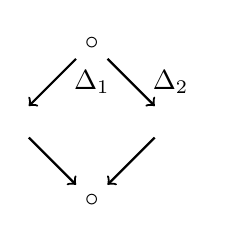
\begin{tikzpicture}
    \draw[thick, ->] (-0.2,-0.2) -- (-0.8,-0.8);
    \draw[thick, ->] (0.2,-0.2) -- (0.8,-0.8);
    \draw[thick, ->] (-0.8,-1.2) -- (-0.2,-1.8);
    \draw[thick, ->] (0.8,-1.2) -- (0.2,-1.8);

    \draw (0,0) node {$\circ$};
    \draw (0,-2) node {$\circ$};
    \draw (0,-0.5) node {$\Delta_1$};
    \draw (1,-0.5) node {$\Delta_2$}; % Add etas on the arrows
  \end{tikzpicture}
\end{center}
\textbf{Proof of (2):} Consider how $\Delta_1$ and $\Delta_2$ overlap. There can be no conflict.

\begin{enumerate}[(3)]
  \item Eta expansion has strong diamond
  \item Eta expansion has Church-Rosser
\end{enumerate}

\subsection{Eta expansion of terms with potential}
\begin{equation*}
  U^{\alpha,n+1,n+2,\beta} \stackrel{\hbox{\tiny eta expansion}}{\longrightarrow} (\l u^{n+1} (U^{\alpha,n+1}u^{n+1,n})^{n,n+1})^{n+2,\beta}
\end{equation*}